%!TEX root = francis_thesis.tex
%%%%%%%%%%%%%%%%%%%%%%%%%%%%%%%%%%%%%%%%%%%%%%%%%%%%%%%%%%%%%%%%%%%%%%%
\chapter{Results and analysis}\label{ch:Results}


\section{Used Technologies}
Various technologies, frameworks and libraries were used in this project. Every implementation was carried out in Python, and frameworks like TensorFlow and Keras were used. Below are the list of the technologies used and a brief description.

\subsection{Python}

\begin{figure}[H]
    \centering
    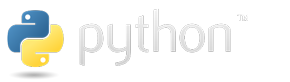
\includegraphics[width=0.8\linewidth]{images/python-logo.png}
     \caption{Python logo, source: https://www.python.org/community/logos/}
  \end{figure}

Python\footnote{https://www.python.org/community/logos/} is a high level programming language designed by Guido van Rossum in 1991. Its design philosophy emphasizes code readability and has a remarkable use of significant whitespace. The filename extensions include .py, .pyc, .pyw, .pyz. It support web development with frameworks like Django and Pyramid. It is applied in scientific studies and machine learning. Several libraries and frameworks have been developed by the Python community for this such as 
SciPy\footnote{www.scipy.org}, Scikit-learn\footnote{scikit-learn.org/stable/}, Pandas\footnote{pandas.pydata.org}, Numpy\footnote{www.numpy.org/}, Theano\footnote{deeplearning.net/software/theano/}, PyTorch \footnote{pytorch.org/}, etc. It is also one of the most popular languages in the field of Convolutional neural network. Neural Networks like ResNet, VGGNet, Faster R-CNN, AlexNet in Keras or Pytorch, etc. 

\subsection{ TensorFlow}
\begin{figure}[H]
    \centering
    
\includegraphics[width=0.7\linewidth]{images/TensorFlow.png}
     \caption{TensorFlow logo, source: www.tensorflow.org}
  \end{figure}
TensorFlow\footnote{www.tensorflow.org} is an Apache Licensed library. It is free and open-sourced and developed by Google Brain Team. It is written in Python, C++ and CUDA. It is a symbolic math library applied for machine learning application such as deep neural network, convolutional neural network. TensorFlow was used in the implementation of the deep learning network for this project. TensorFlow has a comprehensive, flexible ecosystem of tools, libraries that makes it user-friendly.
For a wider documentation, please see the official website\footnote{www.tensorflow.org}
\clearpage

\subsection{Keras}
\begin{figure}[H]
    \centering
    
\includegraphics[width=0.9\linewidth]{images/keras.png}
     \caption{Keras logo, source:www.scikit-image.org}
  \end{figure}

Keras \footnote{Keras.io} is an MIT licensed neural-network library written in Python. It was design by Francois Chollet and released first in March 2015. It is open-sourced. Keras is capable of running on top of Microsoft Cognitive Toolkit, TensorFlow, PlaidML or Theano for fast experimentation of deep neural networks. It enables implementation of deep learning and allows easy and 
fast prototyping, supports both convolutional networks and recurrent networks and the combination of both. For a wider documentation, please see the official website\footnote{www.keras.io}

\subsection{ Scikit-Image}
\begin{figure}[H]
    \centering
    
\includegraphics[width=0.7\linewidth]{images/Scikit-image.png}
     \caption{Scikit-Image logo, source: www.scikit-image.org}
  \end{figure}

Scikit-Image is a BSD licensed image processing library. It is a collection of algorithms for segmentation, 
geometric transformations, analysis, filtering, colour space manipulation, morphology, feature detection, and so on. It was first released in 2009, written by Stefan van der Walt.
\cleardoublepage
\section{Implementation}
\subsection{Dataset}
Drones, or general UAVs, equipped with cameras have been fast applied to a wide range of applications, including agricultural, aerial photography, fast delivery, and surveillance. Consequently, automatic understanding of visual data collected from these platforms become highly demanding, which brings computer vision to drones more and more closely. 
Various computer vision task has been carried out by the Vision meets Drone (VisDrone) Challenges\footnote{www.aiskyeye.com}
organized  by the AISKEYE team at Lab of Machine Learning and Data Mining , Tianjin University, China in the year 2018.
Various computer vision task carried out in the challenge include object detection in images. The task aims to detect objects of predefined categories (e.g., cars and pedestrians) from individual images taken from drones. Also, object detection in videos challenge. The task is similar to the first, except that objects are required to be detected from videos. Then single-object tracking challenge. The task aims to estimate the state of a target, indicated in the first frame, in the subsequent video frames. And finally, multi-object tracking challenge. The task aims to recover the trajectories of objects in each video frame.
Originally, I wanted to use the dataset provided by VisDrone Challenge for the training and validation of my Mask R-CNN Network, but due to lack of the segmentation mask data for the training set, I couldn’t use it.
Rather I made use of the Semantic Drone Dataset from Institute of Computer Graphics and Vision, Graz University of Technology, Austria. \footnote{dronedataset.icg.tugraz.at}

\paragraph{}
The dataset contains images, bounding boxes as python pickle file, bounding boxes as xml, bounding boxes as mask images. The Semantic Drone Dataset focuses on semantic understanding of urban scenes for increasing the safety of autonomous drone flight and landing procedures. The imagery depicts  more than 20 houses from nadir (bird's eye) view acquired at an altitude of 5 to 30 meters above ground. A high resolution camera was used to acquire images at a size of 6000x4000px (24Mpx). The training set contains 400 publicly available images and the test set is made up of 200 private images. [W]
For the task of person detection the dataset contains bounding box annotations of the training and test set. And for semantic segmentation, pixel-accurate annotation for the same training and test set was prepared. The complexity of the dataset is limited to 20 classes as listed below.

\begin{itemize}
  \item tree
  \item tree
  \item grass
  \item other vegetation
  \item dirt
  \item gravel
  \item rocks
  \item water
  \item paved area
  \item pool
  \item person
  \item dog
  \item car
  \item bicycle
  \item roof
  \item wall
  \item fence
  \item fence-pole
  \item window
  \item door
  \item obstacle
  
\end{itemize}
The Drone Dataset is made freely available to academic and non-academic entities for non-commercial purposes such as academic research, teaching, scientific publications, or personal experimentation.
\paragraph{}
For the implementation of the instance segmentation, Python was used for obvious reasons. It enabled me to use deep learning framework like Tensorflow and Keras. The implementation of the model was carried out in the file drone.py and uses the Mask R-CNN library developed in python with TensorFlow and Keras by Matterport Inc. It was written by Waleed Abdulla from Matterport Inc. Matterport, Inc. published their implementation under the MIT License \cite{X}. The MIT License is a license granting the permission to use the code, copy it, modify it, publish and even to sell it free of charge.
There's absolutely no restriction on commercial use in MIT license. The only requirement is that you must include the MIT copyright notice with any copies of the software. Scripts, files and noteboks in the library are also under the MIT License and moreover, Waleed Abdulla himself agreed with the usage and modifications of his code for purposes of the research work.The Matterport, Inc. Mask R-CNN implementation can be found in their GitHub repository.
Moreover, the Matterport implementation of Mask R-CNN was selected because of several reasons. Besides its license compatibility, it is quite robust and ready for modifications and adaptation for training in drone dataset leading to another implementation, so it saved thousands of lines of code. One of the major motivation behind its usage is that there is a plenty of people interested in this project, proposing their ideas and testing it. And these people are experienced in fields of computer vision and deep learning. Abdulla himself is responsive and active in answering people’s questions and issues. He is open-minded when discussing other people improvement proposals. I found it very useful.
The next section will discuss the Mask R-CNN library, the workflow and necessary module of the library. The structure, architecture and components of the Mask R-CNN have been discussed in Chapter 2, so explanation of the programs only will be given in the next section. The library will be also discussed altogether with notes on my modifications connected with this thesis to distinguish them from Abdulla’s code.

\subsection{Mask R-CNN library}
The library which is hosted in Github has been forked 5445 times. It contains five important modules. Each module play an important role in the training and testing of model. Let’s go through this modules on after the other below:
\\
\textbf{Config.py}
\\
This is the configuration module of the system. It includes hyper-parameters for tuning of the model and necessary setting. It will described in section 4.2.1SS
\\
\textbf{Model.py}\
This is fundamental core of the model. It develops and builds up the model. It will described in section 4.2.2
\\	
\textbf{Parallel\_Model.py}\ 
This module subclasses the standard Keras Model and adds multi-GPU support. It works by creating a copy of the model on each GPU and creates a parallelized computation.
This file was not modify further and so will not explained in this thesis.
\\
\textbf{Utils.py} \
This modules contains the utility classes and functions of the model. It will described in section 4.2.3
\\
\textbf{Visualize.py}\
This contains function for display and visualization. It will described in section 4.2.4
\\

The python files for the modules have good inner documentation, of which some of them and other functionalities will be discussed next.

\subsubsection{Config.py}
Config.py is the configuration settings for the model in the implementation by Matterport Inc.. It contains the hyper-parameters of the model. It has a classed called ModelConfig that houses these parameters. These parameter include;
 \begin{itemize}
   \item GPU Count
   \item Images per GPU
   \item Steps per Epoch
   \item Validation steps
   \item The choice of the backbone
   \item Backbone strides (The strides of each layer of the Feature Pyramid Network (FPN) pyramid discussed in section 2.2)
   \item Learning Rate
   \item RPN Train Anchors Per\_ Image (How many anchors per image to use for RPN training)
   \item Mask Shape
   \item And so on.
   
 \end{itemize}
 I inherited ModelConfig  class and then adapted the attributes to suit my hardware and the drone-based dataset in the drone.py module.  The config.py also a contains a display function that displays the model’s attribute.

 \subsubsection{Model.py}
 This is the main Mask R-CNN implementation. It is made use of some modules for its implementation which include, os, random, datetime, re, logging, collections, multiprocessing ,numpy,tensorflow, keras, keras.backend ,keras.layers ,keras.engine  ,keras.models. distutils.version. For the module to work it needs TensorFlow 1.3+ and Keras 2.0.8+ .  Since this module builds the Mask R-CNN it has several classes and function performing various tasks. This classes and task the perform can be summed up thus;
 \begin{itemize}
   \item 	Initialization functions
   \item Building the ResNet backbone.
   \item Building the RPN.
   \item Building RoIAlign layers.
   \item Building head architectures.
   \item Building the complete Mask R-CNN model and putting everything together.
   \item Building detection layers.
   \item Defining loss functions.
   \item	Data formatting
   \item Miscellaneous functions and utilities connected to the model, like batch normalization data formatting and generating (building up targets, loading ground truth masks) or bounding boxes normalization.
   
 \end{itemize}
 Some important functions in the modules include train, load\_weight, build, etc. There was no modification made in this module for the training of model, apart from few modification to fix error that could be raised during the loading of masks. An explanation is given to the program written by Waleed Abdulla
\\ 
\\
\textbf{ RESNET}
\\
 The backbone of the Mask R-CNN is the Residual Network (RESNET). For the building of the RESNET, the principal function that does this is the resnet\_graph . The  resnet\_graph builds the ResNet graph and the  architecture can be ResNet50 or ResNet101.The batch norm layers of the network can be freeze or trained by setting the train\_bn to True or False, but the default is True. The workflow is outlined in pseudocode 4.1
 \\
\\

 \begin{algorithm}[H]
  \caption{Building the ResNet backbone architecture}
  \SetAlgoLined
  \DontPrintSemicolon
 layers = intended layers\;
 layers .add( zero padding 3x3)\;
 layers .add( convolution 7x7)\;   
 layers .add( batch normalization )\;
 layers .add( ReLu )\;
 layers .add( maximum pooling )\;
 layers .add( convolutional block 64 x64x256 )\;
 layers .add (2 identity blocks 64 x64x256 )\;
 layers .add( convolutional block 128 x128x512 )\;
 layers .add (3 identity blocks 128 x128x512 )\;
 layers .add( convolutional block 256 x256x1024 )\;
\uIf{architecture == ’resnet50 ’}{
  layers .add (5 identity blocks 256 x256x1024 )\;
}
\uElseIf{architecture == ’resnet101 ’}{
  layers .add (22 identity blocks 256 x256x1024 )\;
}


\textbf{return} layers\;   
 \end{algorithm}
.\\
\\
The genuine function does not return total layers, however, it returns them in stages  C1, C2, C3, C4, C5 as can be seen in pseudocode 4.8, where this function is called  build\_resnet\_backbone. Every one of these stages speaks to the condition of craftsmanship before each convolutional block expansion, which is the last layer before changing components of input or yields. It is significant for the FPN as was referenced in Chapter 2 what's more, outlined in the model structure in pseudocode 4.8. Functions identity block and convolutional block are fundamentally the same as and both fabricates the bottleneck block. The main contrast is that the convolutional block function likewise actualizes a 1x1 convolution in the alternate route association as it is important to change the state of the contribution to the one utilized in the block. The remainder of their usage is pretty much the equivalent and is represented in pseudocode .2 (the convolution ought to be connected in the yield association step). It uses channels given to each call of the capacity in the ResNet pseudocode.
\\
\\
\begin{algorithm}[H]
  \caption{identity\_block}
  \SetAlgoLined
  \DontPrintSemicolon
  original\_input = original\_input\_tensor\;
  block = intended block of layers\;
   block .add ( convolution 1x1)\;
   block .add ( batch normalization )\;
   block .add ( ReLu )\;
   block .add ( convolution 3x3)\;
   block .add ( batch normalization )\;
   block .add ( ReLu )\;
   block .add ( convolution 1x1)\;
    block .add ( batch normalization )\;
   block . connect\_outputs (block , original\_input )\;
   block .add ( ReLu )\;
   \textbf{return} block\;
  
  \end{algorithm}
.\\
\\
 \textbf{RPN}
\\
The RPN is worked by two functions, build\_rpn\_model and rpn\_graph. Notwithstanding, these functions assemble just the model, for example, the sliding window and its behavior, anchors are created in utils.py as depicted in section 5.1.3. Indeed, even in this split approach, it pursues the thought from section 3.4.3. Contributions for the rpn\_graph capacity are an element map, number of anchors per area and anchors stride and returns anchors class logits, probabilities and bounding boxes refinements. The work process of rpn\_graph is represented in pseudocode 5.3. build\_rpn\_model makes a model which initially feed the rpn\_graph work and at that point restores the previously mentioned qualities.
\\
\\
\begin{algorithm}[H]
  \caption{rpn\_graph}
  \SetAlgoLined
  \DontPrintSemicolon
  feature\_map = input\_feature\_map\;
  logits\_number\_of\_filters = 2 * number of anchors per location\;
   bbox\_number\_of\_filters = 4 * number of anchors per location\;
   shared\_layer = convolution 3x3 on feature\_map\;
   rpn\_class\_logits = convolution 1x1 on shared\_layer with logits\_number\_of\_filters\;
  rpn\_probabilities = softmax on rpn\_class\_logits\;
   rpn\_bbox\_refinements = convolution 1x1 on shared\_layer with bbox\_number\_of\_filters\;
   \textbf{return} rpn\_class\_logits , rpn\_probabilities , rpn\_bbox\_refinements\;
  
  \end{algorithm}
  .\\
\\
  A significant class for the RPN is the ProposalLayer class. It takes anchor probabilities, bounding box refinements and anchors themselves as inputs trim them to littler clumps while considering top anchors and applies refinements to the anchor boxes.
\\
\\
\begin{algorithm}[H]
  \caption{ProposalLayer}
  \SetAlgoLined
  \DontPrintSemicolon

probs = anchor probabilities\;
deltas = anchor refinements\;
anchors = anchors\;
threshold = threshold for probabilities\;
top\_anchors = names\_of\_anchors\_with\_top\_probs (probs , how\_many =min(6000 , len( probs )))\;
 probs\_batch = batch\_slice (probs , top\_anchors )\;
 deltas\_batch = batch\_slice (deltas , top\_anchors )\;
 anchors\_batch = batch\_slice ( anchors , top\_anchors )\;
 boxes = apply\_refinements ( anchors\_batch , deltas\_batch )\;
 proposals = [boxes , probs\_batch ]\;
 proposals . apply\_threshold ( threshold )\;
 \textbf{return} proposals\;

  \end{algorithm}
  .\\
  \\
\clearpage
 \textbf{ROIAlign}
\\
As was described already in chapter 2, RoIAlign is more or less the RoIPooling algorithm without rounding. The implementation is briefly sketched below
\\
\\
\begin{algorithm}[H]
  \caption{RoIAlign}
  \SetAlgoLined
  \DontPrintSemicolon
pool\_shape = shape of regions\;
 image\_shape = shape of the image\;
 boxes = list of RoIs\;
 feature\_maps = list of feature maps\;
 h, w = compute\_heights\_and\_widths\_boxes ( boxes )\;
 image\_area = image\_shape [0] * image\_shape [1]\;
 roi\_level = minimum (5, 4 + log2 ( sqrt (h * w) / (224 / sqrt (image\_area ))))\;
pooled = list ()\;
\For{\texttt{level in range (2, 6)}}{
 roi\_level\_i = 1 where roi\_level == level , 0 elsewhere\;
 level\_boxes = gather (boxes , indices = roi\_level\_i )\;
 pooled . append ( crop\_and\_resize ( original\_image = feature\_maps [level-2] , what\_process = level\_boxes , shape = pool\_shape , method =’
bilinear ’))\;}

pooled . rearrange\_to\_match\_the\_order ( boxes )\;
\textbf{return} pooled\;
\end{algorithm}
.\\
\\
It executes the RoIAlign algorithm on different dimensions of the feature pyramid furthermore, in its specifications of the \newcommand*{\logten}{\mathop{\log_{2}}} condition, it pursues the thoughts behind identifications in [27] and furthermore applies the five-levels approach. The base picking at line 7 and the loop at line 9 the then pursues utilizing just layers two to five from chapter 5.1.2.
\\
\\
\textbf{Head architectures}
\\
As can be found in figure 3.13 and was at that point portrayed in section 3.6.1, the head architecture is separated into two areas. The head architecture for bounding boxes what's more, class probabilities are dealt with by the fpn\_classifier\_graph function and the mask architecture by the build\_fpn\_mask\_graph. 
fpn\_classifier\_graph takes as input RoIs, feature maps, pool size and a number of classes and returns classifier logits, probabilities and bounding boxes refinements. build\_fpn\_mask\_graph takes a similar input yet returns just a rundown of masks.
\\
\\
\begin{algorithm}[H]
  \caption{fpn\_classifier\_graph}
  \SetAlgoLined
  \DontPrintSemicolon
  rois = given regions of interest in normalized coordinates\;
  feature\_maps = list of feature maps from layers P2 , P3 , P4 , P5\;
   pool\_size = height of feature maps to be generated from ROIpooling\;
  num\_classes = number of classes\;
  layers = list of keras layers\;
  layers .add( ROIAlign ( pool\_size , input =[ rois , feature\_maps ]))\;
   layers .add( convolution pool\_size X pool\_size )\;
   layers .add( batch\_normalization )\;
   layers .add( ReLU )\;
   layers .add( convolution 1x1)\;
   layers .add( batch\_normalizataion )\;
   layers .add( ReLU )\;
   shared = squeeze\_to\_one\_tensor ( output of layers )\;
   class\_logits = fully\_connected\_layer ( input =shared ,number\_of\_filters = num\_classes )\;
   probabilities = softmax ( class\_logits )\;
   bboxes = fully\_connected\_layer ( input =shared , number\_of\_filters =4 * num\_classes )\;
   return class\_logits , probabilities , bboxes\;
  
  
\end{algorithm}
.\\
\\
\begin{algorithm}[H]
  \caption{build\_fpn\_mask\_graph}
  \SetAlgoLined
  \DontPrintSemicolon
   rois = given regions of interest in normalized coordinates\;
   feature\_maps = list of feature maps from layers P2 , P3 , P4 , P5\;
   pool\_size = height of feature maps to be generated from ROIpooling\;
   num\_classes = number of classes\;
   layers = list of keras layers\;
   layers .add( ROIAlign ( pool\_size , input =[ rois , feature\_maps ]))\;
   layers .add( convolution 3x3)\;
   layers .add( batch\_normalization )\;
   layers .add( ReLU )\;
   layers .add( convolution 3x3)\;
   layers .add( batch\_normalization )\;
   layers .add( ReLU )\;
   layers .add( convolution 3x3)\;
   layers .add( batch\_normalization )\;
   layers .add( ReLU )\;
   layers .add( convolution 3x3)\;
   layers .add( batch\_normalization )\;
   layers .add( ReLU )\;
   layers .add( deconvolution 2x2 with strides 2)\;
   layers .add( convolution 1x1 with sigmoid as an activation function )\;
  
   \textbf{return} layers
\end{algorithm}
.\\
\\

In the pseudocodes above, a ROIAlign object is added as the first one into layers. This object was sketched in pseudocode 5.5.
\\
\\
\textbf{Mask R-CNN model}
\\
The focal point of the model.py record is the MaskRCNN class which contains techniques to manufacture the whole Mask R-CNN model by cobbling together various kinds of layers 
what's more, to utilize it for training or detection. The work process of the technique build is represented in pseudocode 5.8 and pursues 
the architecture portrayed in chapter 3.6.1. In the pseudocode, we can see that the head architecture contrasts a bit in the training and in the detection. It is expected to 
the way that we need loss values to be processed during the training, so we figure them from detected values and target values (values dependent on known focuses from 
the training dataset).
\\
\\
\begin{algorithm}[H]
  \caption{Mask R-CNN.build}
  \SetAlgoLined
  \DontPrintSemicolon
 C2 , C3 , C4 , C5 = build\_resnet\_backbone ()\;
 P5 , P4 , P3 , P2 = build\_top\_down\_fpn\_layers (C2 , C3 , C4 , C5)\;
 anchors = generate\_anchors ()\;
 rpn = build\_rpn ()\;
 rois = ProposalLayer (rpn , anchors )\;
 \eIf{ mode == 'training '}{
    ground\_truth\_values = values from the training dataset\;
    bbox , classes = fpn\_classifier ( rois )\;
    target\_detection = DetectionTargetLayer ( ground\_truth\_values )\;
  mask = fpn\_mask ( rois from target\_detection )\;
   loss = loss\_functions ( target\_detection , bbox , classes , mask )\;
   model = [bbox , classes , mask , loss ]\;
}{
     bbox , classes = fpn\_classifier ( rois )\;
     target\_detection = DetectionLayer (bbox , classes )\;
     mask = fpn\_mask ( rois )\;
    model = [bbox , classes , mask ]\;
 }
 \textbf{return} model\;
\end{algorithm}
.\\
\\ 
In the pseudocode, we can see a few classes and functions. Despite the fact that their motivations are very clear, some of them can be seen in various pseudocodes. Function
build\_resnet\_backbone was at that point depicted in pseudocode 5.1, ensuing function build\_top\_down\_fpn\_layers is genuinely clear procedure connecting layers 
as in section 3.6.1, generate\_anchors will be portrayed in 5.12, build\_rpn can be seen in pseudocode 5.3, ProposalLayer in pseudocode 5.4, fpn\_classifier speaks to the fpn\_classifier\_graph from pseudocode 5.6 and fpn\_mask is work 
build\_fpn\_mask\_graph from pseudocode 5.7.

\subsubsection{utils.py}
The most significant piece of the utils.py record is the Dataset class. It is likewise the main 
some portion of the utils.py code that was adjusted for the necessities of Drone-based dataset utilization 
(the other changes are simply minor refactorings). The utils.py additionally contains a great deal of functions. Just a couple of them will be referenced 
as every one of them have adequate documentation in the code.
\\
\\
\textbf{Dataset}
\\
The Dataset class is the base class for dataset classes and images. It contains data about them including their names, identifiers and on account of images

likewise paths to them. One of the written methods is the one called import\_contents, which feeds the Dataset object with classes and images. The work process is represented in pseudocode 

5.9. Contributions for the technique are: 
\begin{itemize}
  \item List of classes names proposed to be learned

  \item List of directories containing training images and masks 
  \item Name of model
\end{itemize}

The add\_class method in pseudocode 5.9 import a class into the Dataset object dictionary  inside and out with an exceptional identifier; a significant part is containing 
the foundation as the first class with identifier 0 (in the pseudocode represented simplifiedly by the saved\_class dictionary ). The add\_images line is a loop over all 
images with the predefined augmentation contained in a given registry bringing in them out and out with their identifier and way into the Dataset object list.
\\
\\
\begin{algorithm}[H]
  \caption{import\_contents}
  \SetAlgoLined
  \DontPrintSemicolon
   classes = list of classes names intended to be learned\;
  directories = list of directories containing training images and
  masks\;
  saved\_classes = {’BG ’: 0}\;
  \For{\texttt{ i in classes}}{
   add\_class\;}
   \For{\texttt{ directory in directories}}
   {add\_images\;}
  
\end{algorithm}
.\\
\\ 
Another important method written for the needs of the Drone-based dataset modules is
the one called load\_mask. The work process of the method is illustrated in pseudocode
5.10. It returns an array containing boolean masks (True for the mask, False elsewhere)
for each instance in the image, an array of class identifiers corresponding each instance in the masks array.
\\
\\
\begin{algorithm}[H]
  \caption{get\_mask}
  \SetAlgoLined
  \DontPrintSemicolon
masks\_list = list of mask files within the directory\;
first\_mask = masks\_list [0]\;
masks\_array = array containing first\_mask transformed to bool\;
classes\_list = list containing class of the first mask\;
\For{\texttt{  new\_mask in masks\_list [1:]}}{
 concat\_mask = new\_mask transformed to bool\;
 concatenate masks\_array with concat\_mask\;
 append class of new\_mask into classes\_list\;
 \uIf {any problem happened}
 {\textbf{return} None , None\;}
}
\textbf{return} masks\_array , classes\_list\; 
\end{algorithm}
.\\
\\
From the remainder of Dataset class methods, one more will be referenced. prepare must be called before the use of the Dataset object as it sets it up for use. 
The readiness is done through setting object parameters like number of classes, classes names and identifiers or number of pictures. This setting depends on 
data got during the import\_contents call. Bounding boxes apparatuses Since bounding boxes are not required to be given altogether with masks
in the training dataset, the function extract\_boxes is utilized to process bounding boxes from masks. The function scans for the first and last horizontal and vertical 
positions containing mask along all channels and returns them as an array. It implies that every pixel of the mask is contained in the returned horizontal-vertical bounding 
box and it is likewise as tight as could reasonably be expected. 
A function used to register the IOU is called just compute\_iou. Its work process is delineated in pseudocode 5.11. The treatment of no interception is likewise executed 
in the function, yet for better understanding, it is excluded in the pseudocode. 
\\
\\
\begin{algorithm}[H]
  \caption{compute\_iou}
  \SetAlgoLined
  \DontPrintSemicolon
   predicted\_box\_area = area of predicted box\;
groundtruth\_box\_area = area of given mask\;
y1 = the bigger one from the upper coordinates of the predicted and ground truth bboxes\;
 y2 = the smaller one from the lower coordinates of the predicted and ground truth bboxes\;
x1 = the bigger one from the left coordinates of the predicted and ground truth bboxes\;
x2 = the smaller one from the right coordinates of the predicted and ground truth bboxes\; 
intersection = (x2 - x1) * (y2 - y1)\;
union = predicted\_box\_area + groundtruth\_box\_area - intersection\;
iou = intersection / union\;
\textbf{return} iou
\end{algorithm}
.\\
\\
With the correlation of ground truth boxes and the anticipated ones is associated likewise the function box\_refinement. It registers contrasts between ground truth 
furthermore, anticipated directions of bounding boxes and returned them as the data 
of the error bounding box incorrectness. 
\\
\\
\textbf{Pyramid anchor tools }
\\
The hypothesis of scales and pyramids was at that point portrayed in chapter 3.4.3 and 3.6.1. Two functions  are associated with the formation of the anchors at various dimensions of 
a feature pyramid. The called one is generate\_pyramid\_anchors which loops over scales. Tuned in, the generate\_anchors capacity is called to produce anchors of 
proportions for a given arrangement of scales. The work process of the generate\_anchors function is represented in pseudocode 5.12. It takes scales and proportions of anchors, feature map shape and anchors and 
feature map strides as a series of inputs. It utilizes these contributions to figure heights and widths of various stays (can be found in figure 3.6) and to compute a framework of anchors
focuses. This network together with their height and widths characterizes the returned value, anchors.
\\
\\
\begin{algorithm}[H]
  \caption{generate\_anchors}
  \SetAlgoLined
  \DontPrintSemicolon
  scales = array of scales\;
ratios = array of ratios\;
feature\_map\_shape = [height , width ]\;
anchor\_stride = stride of anchors on the featuremap\;
feature\_stride = stride of the featuremap\;
 heights = scales divided by a square root of ratios ( each by each )\;
 widths = scales multiplied by square root of ratios ( each by each )\;
 shifts\_y = grid from 0 to shape [0] with stride anchor\_stride\;
 shifts\_y = shifts\_y * feature\_stride\;
 shifts\_x = grid from 0 to shape [1] with stride anchor\_stride\;
 shifts\_x = shifts\_x * feature\_stride\;
 anchors\_centers = stack of [ shifts\_y , shifts\_x ] in each combination\;
anchors\_sizes = [ heights , widths ]\;
anchors = [ anchors\_centers - 0.5 * anchors\_sizes , anchors\_centers + 0.5 * anchors\_sizes ]\;
\textbf{return} anchors
\end{algorithm}
.\\
\\
\textbf{Drone.py}
The responsibility of parents in teaching and training their children. The responsibility of drone.py is to train the model to detect or 
predict object. Drone.py teaches the model to recognize the object attributes, colour, curves, edges and other attributes of object. 
This file was written as part of the practical section of the thesis and defines an important function- train. 
The train function in drone.py calls the parent train function present in the Mask R-CNN model defined above.  Before the training can take place the dataset needs to be loaded and likewise the mask. So the call to the load\_drone function loads the drone-bades dataset and their corresponding mask.   
After the load\_drone function the next is the call to the prepare function. The prepare function sets up the model for training.
The flowchart contains couple of as of now referenced functions and classes, explicitly the ModelConfig class and its display method from chapter 5.1.1, the MaskRCNN 
class from section 5.1.2 and the Dataset class and its methods import\_contents what's more, prepare from chapter 5.1.3. 
The last advance in this flowchart, a method model.train(), has really two extraordinary structures relying upon the utilization of initial weights. The initial structure is connected 
for a training from a scratch and prepares all layers. The second one comprises of three littler sections; right off the bat preparing layers 5 and higher, at that point adjusting layers 4 and 
higher and the last and greatest section is tweaking the entire design. It is appeared in the flowchart in \ref{fig:drone} and the thought behind this conduct is that it is 
unrealistic to train the first layers including low-level features, while changes have a tremendous effect on more profound dimensions and those highlights ought to be pretty much the equivalent for any object.
\clearpage
\begin{figure}[H]
  \centering
  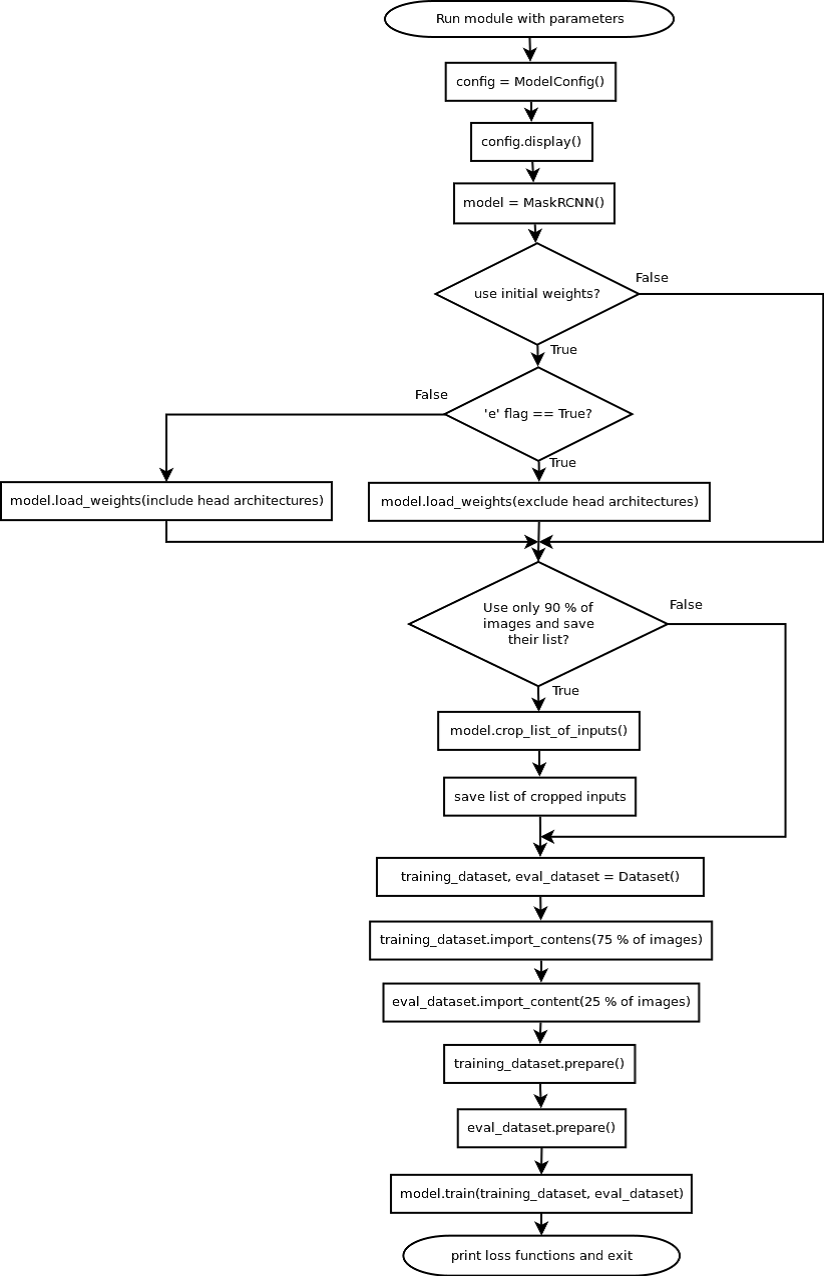
\includegraphics[width=0.8\linewidth]{images/drone-graph.png}
  \caption{Flowchart of the drone.py module written by the author.}
 \end{figure}
 \label{drone}
 \clearpage

 \begin{figure}[H]
  \centering
  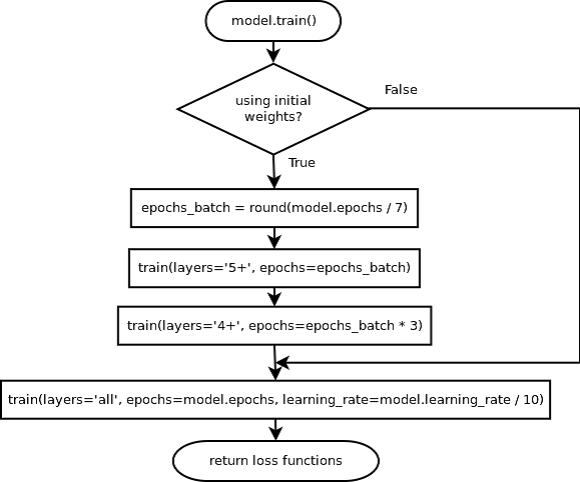
\includegraphics[width=0.8\linewidth]{images/train-graph.png}
  \caption{Flowchart of the train method inside the drone.py module .}
 \end{figure}
 \label{train}
 \clearpage

\textbf{Drone-detect.py}
In the event that we have a trained model, either prepared by us or given by another person, we can utilize it to distinguish highlights or items in maps. In fact, the trained model is used to detect features and maps in drone datasets collected from drones developed by the Robotic Team of African University of Science and Technology.  The yield from 
the module comprises of a set of vector maps for each class. Despite the fact that the model is somewhat scale-invariant, it is prescribed to give object detection and masks incomparable 
goals to the one utilized in training pictures.  The module is contained in the document drone\_detect.py. This record can be viewed as the second piece of the down to earth 
segment of the theory. Its work process is with certain improvements. As in the drone.py module, the flowchart contains few already mentioned 
functions and classes, explicitly the ModelConfig class  and the MaskRCNN class. Be that as it may, more unmentioned function can be found in the detection module.  

